This chapter will describe the requirements of the application as a whole. The structure of this chapter follows the SRS Template as proposed by Wiegers in Chapter 11 and Appendix D of \cite{wiegers2013software}.

\section{Vision and Scope}

    This section describes the high levels goal of the Melanoma Detection App as well as to define boundaries that limit what can be expected of the App.

    \subsection{Business Case}

        A smart phone based assistant would provide a valuable service by making it easy, painless, inexpensive, and fast to get a preliminary risk assessment of a skin lesion. It is too easy to postpone making an appointment with a dermatologist to have a suspect lesion examined. Visiting a dermatologist is not on most people’s list of fun things to do, it requires time and effort. By the time a lesion is visually compelling enough, it might be too late.

A smart phone based application that could make a preliminary diagnosis in near realtime would be a great time save and offer compelling enough information to actually make the appointment with a dermatologist.

    \subsection{Scope and Limitations}

    This chapter describes which features are part of the scope of the Melanoma Detection Application, what can be expected of it, and what are it's limitations.

    \subsubsection{Major Features}
        \noindent
        \begin{itemize}[leftmargin=*]
            \item[]  \textbf{FE-1} : The smart phone app allows the user to capture and analyse an image of a skin lesion and provide a risk assessment to the user of the lesion being a malignant melanoma.

            \item[] \textbf{FE-2} : The app allows the user to create, view, edit or delete metadata that is associated with an image and corresponding risk assessment.

            \item[] \textbf{FE-3} : The app allows the user to save or archive the image and corresponding assessment for future comparison and review.

            \item[] \textbf{FE-4} : The user can browse archived images, assessments, and associated metadata.

            \item[] \textbf{FE-5} : The user can send a set of images with associated assessment and metadata via email.

            \item[] \textbf{FE-6} : The app will run on all popular smart phone devices and systems.

            \item[] \textbf{FE-7} : The analysis algorithms employed by the app should be easily updatable and extendable.
        \end{itemize}

        \begin{figure}[H]
            \centering
            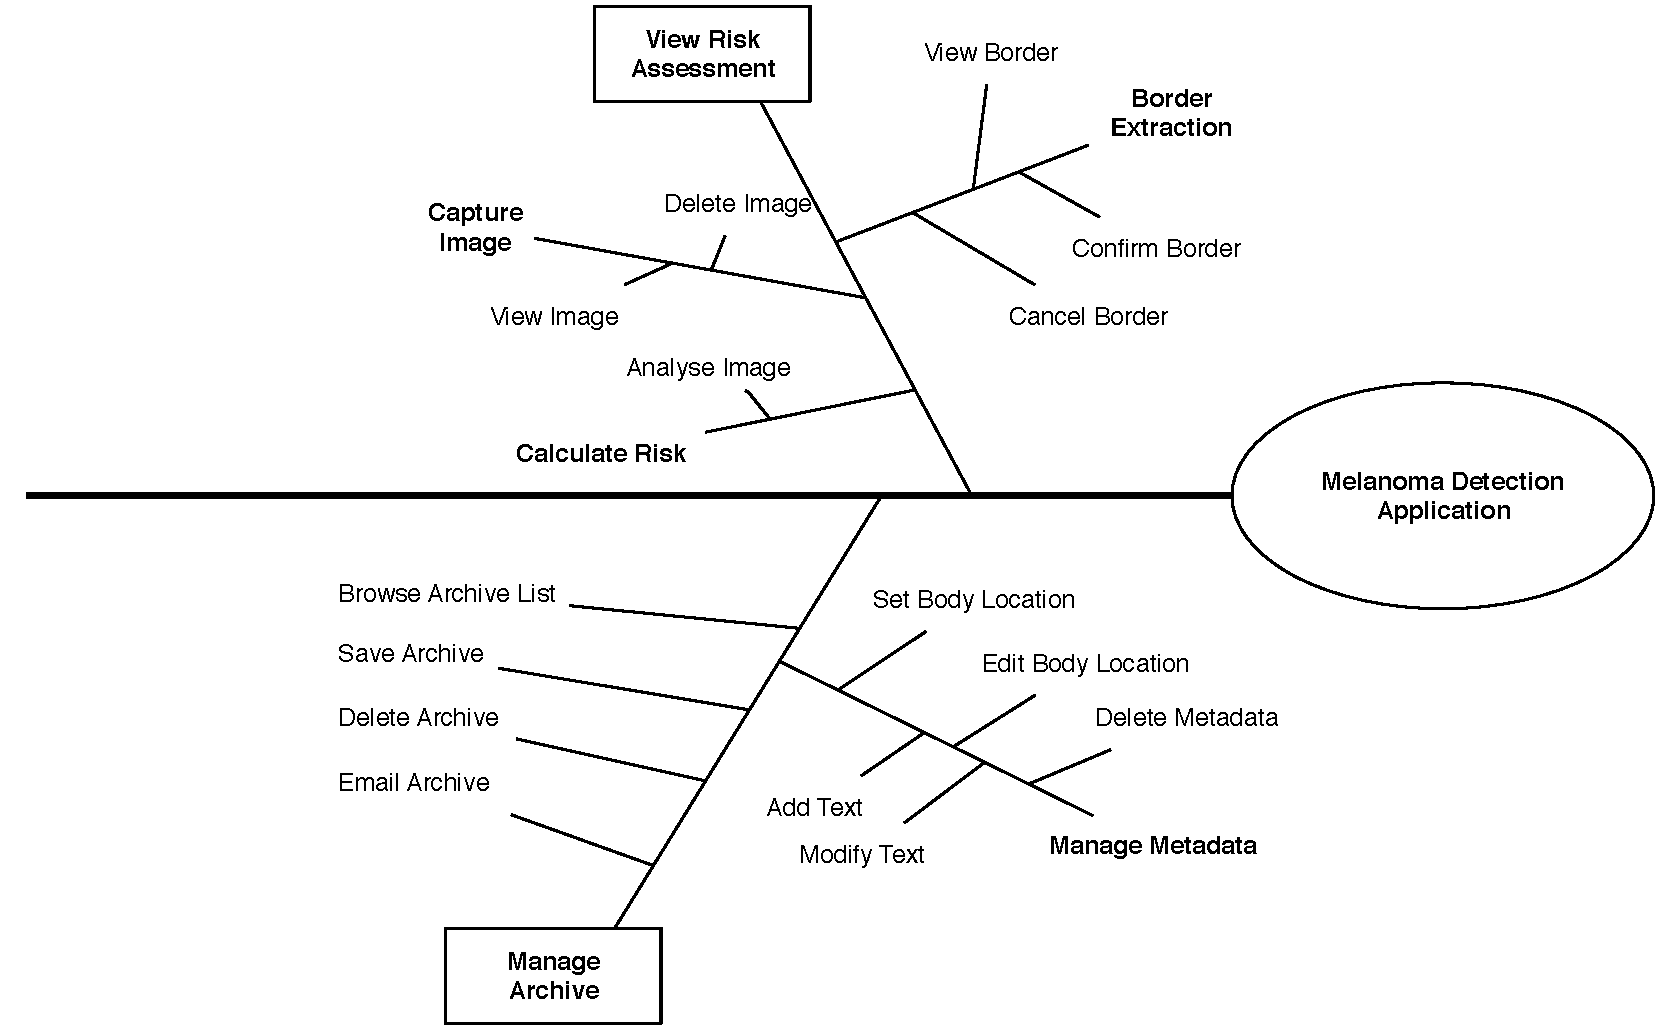
\includegraphics[width=\textwidth]{assets/requirements/PartialFeatureTree.pdf}
            \caption{Partial Feature Tree for the Melanoma Detection App}
            \label{fig:partial_feature_tree}
        \end{figure}

    \subsubsection{Limitations and Exclusions}

        \noindent
        \begin{itemize}[leftmargin=*]
            \item[]  \textbf{LI-1} : The Melanoma Detection App will use visual indicators to calculate the risk of a lesion being a dangerour melanoma. Other types of skin cancer such as basal call carcinoma or squanous cell carcinoma have different characteristics making them less easy to visually detect. The Melanoma Detection App will not take any other types of skin cancer or skin conditions into acount when calculating the risk assessment for melanoma.

        \end{itemize}

    \subsubsection{Stakeholder Profile}

        % TODO

    \subsection{Use Cases}

        10 Important Use Cases have been identified. The schema as defined in Chapter 8 and Appendix D of \cite{wiegers2013software} was used to capture the attributes of each Use Case. The Use Case UML diagram in figure \ref{fig:uml} illustrates the most important use cases. Tables \ref{fig:uc-1} to \ref{fig:uc-10} describe the use cases in detail.

        \begin{figure}[H]
            \centering
            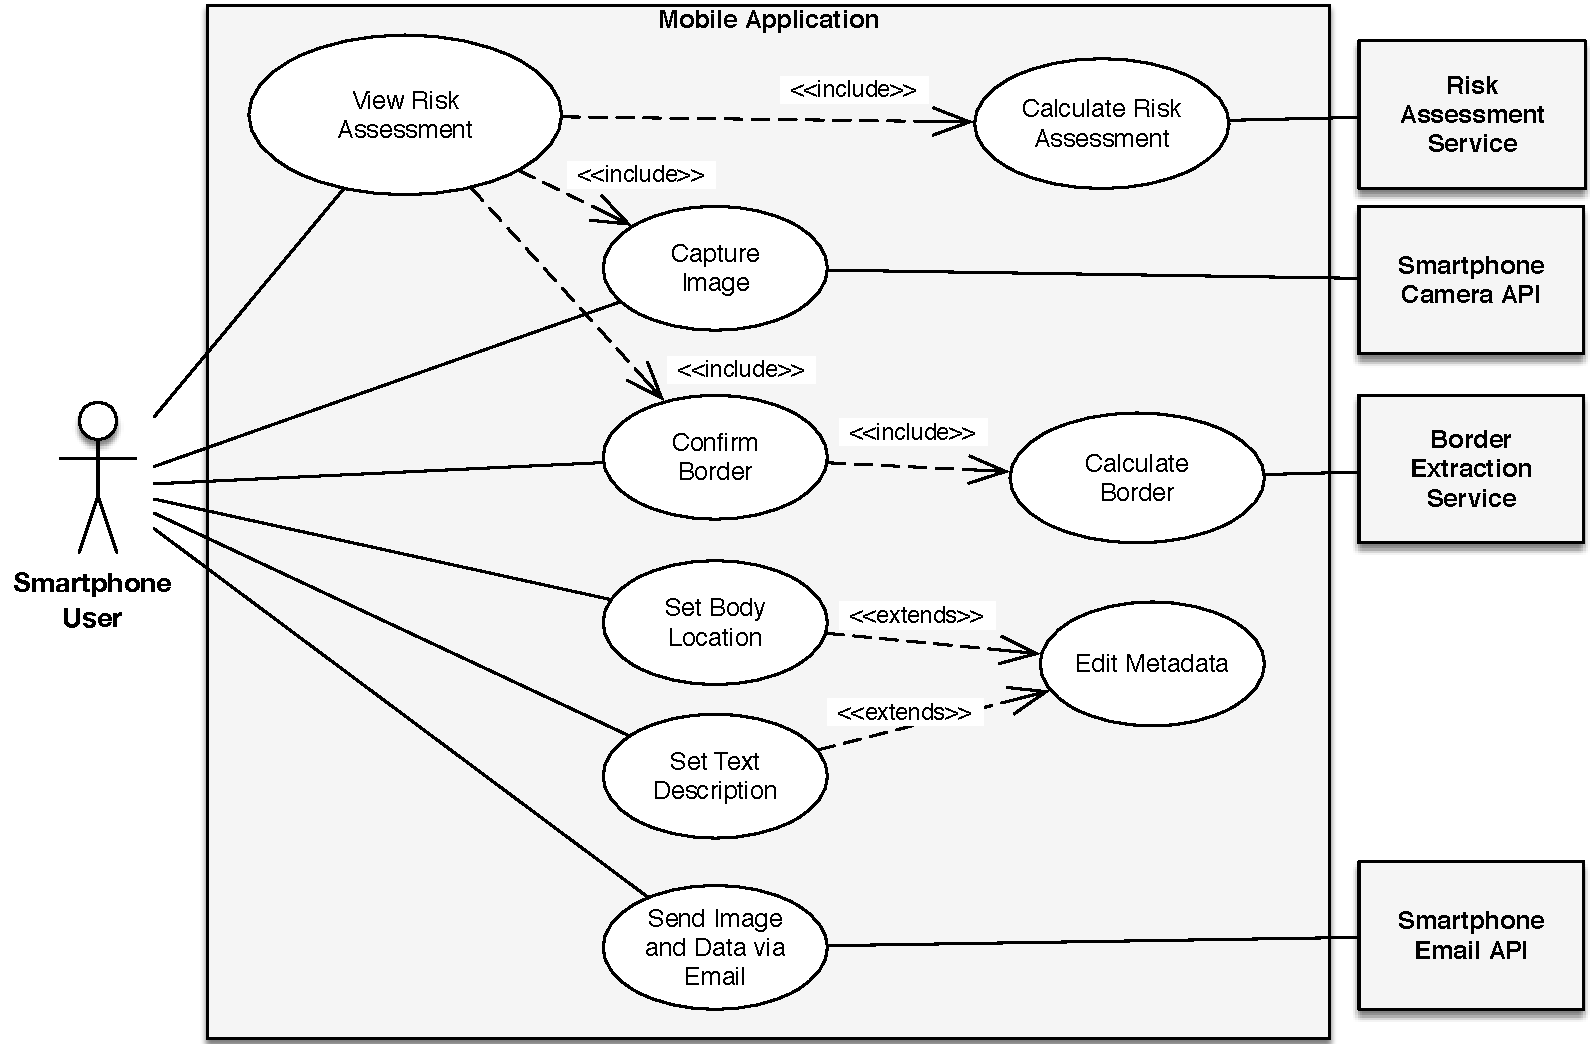
\includegraphics[width=\textwidth]{assets/requirements//uc/UML.pdf}
            \caption{Use Case UML diagram}
            \label{fig:uml}
        \end{figure}

                \begin{table}[H]
            \centering
            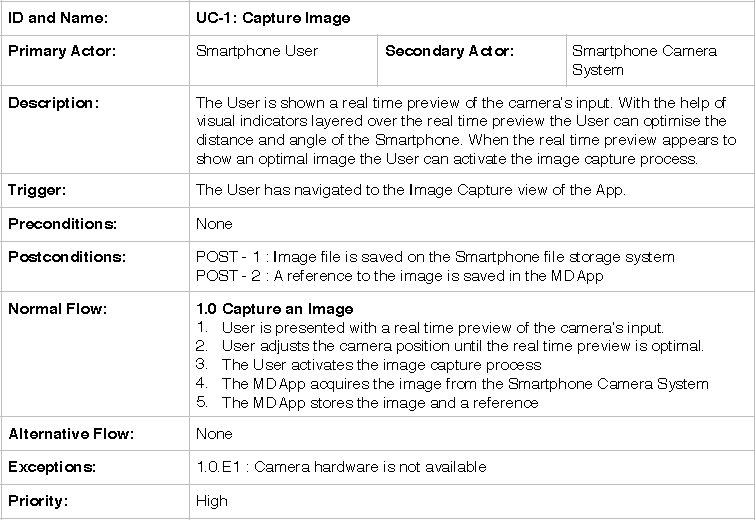
\includegraphics[width=\textwidth]{assets/requirements/uc/usecase_01.pdf}
            \caption{UC-1}
            \label{fig:uc-1}
        \end{table}
        \begin{table}[H]
            \centering
            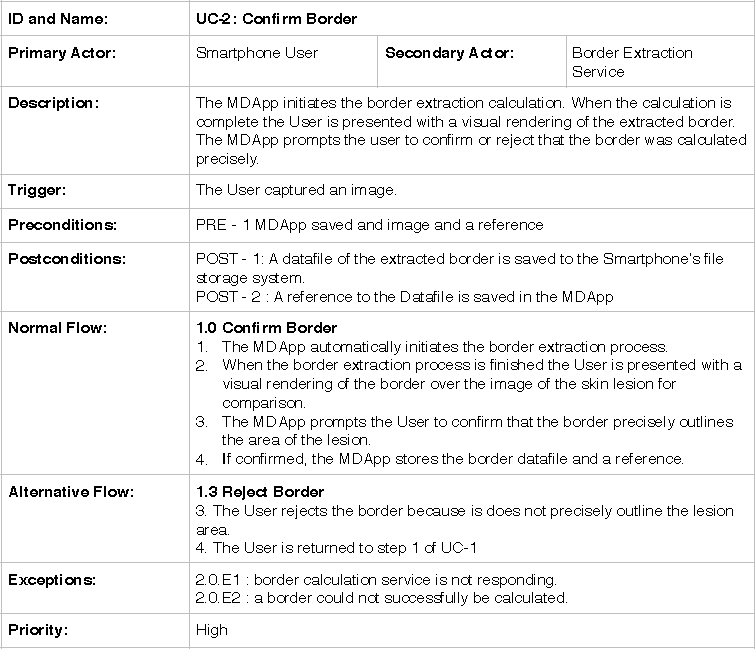
\includegraphics[width=\textwidth]{assets/requirements/uc/usecase_02.pdf}
            \caption{UC-2}
            \label{fig:uc-2}
        \end{table}
        \begin{table}[H]
            \centering
            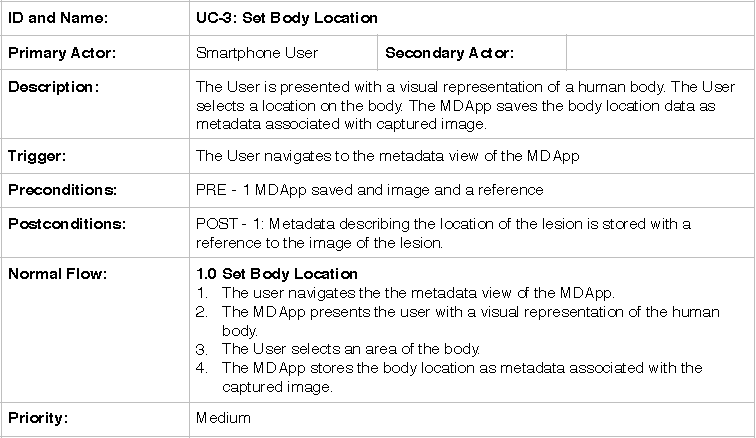
\includegraphics[width=\textwidth]{assets/requirements/uc/usecase_03.pdf}
            \caption{UC-3}
            \label{fig:uc-3}
        \end{table}
        \begin{table}[H]
            \centering
            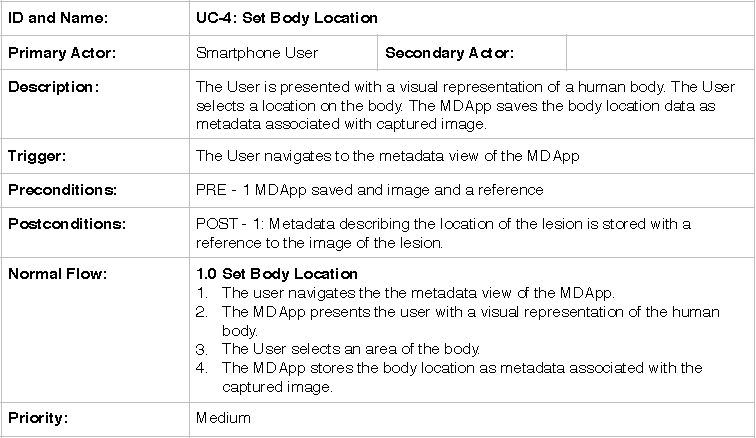
\includegraphics[width=\textwidth]{assets/requirements/uc/usecase_04.pdf}
            \caption{UC-4}
            \label{fig:uc-4}
        \end{table}
        \begin{table}[H]
            \centering
            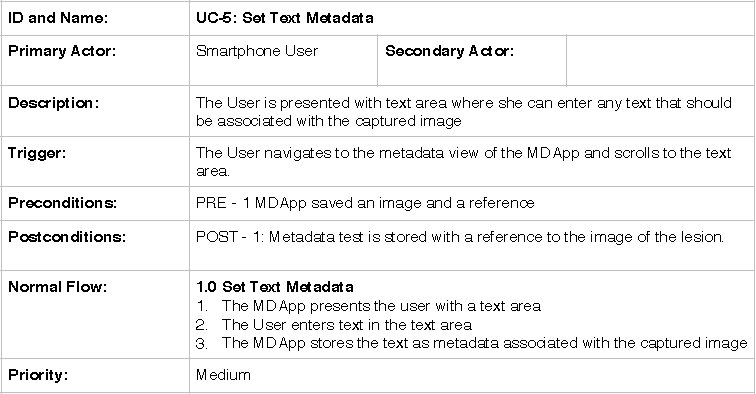
\includegraphics[width=\textwidth]{assets/requirements/uc/usecase_05.pdf}
            \caption{UC-5}
            \label{fig:uc-5}
        \end{table}
        \begin{table}[H]
            \centering
            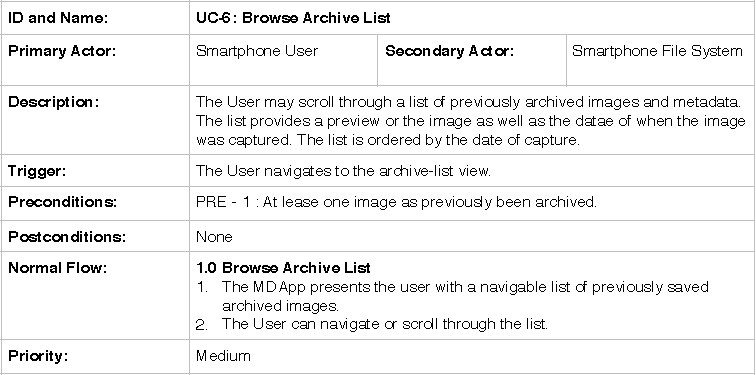
\includegraphics[width=\textwidth]{assets/requirements/uc/usecase_06.pdf}
            \caption{UC-6}
            \label{fig:uc-6}
        \end{table}
        \begin{table}[H]
            \centering
            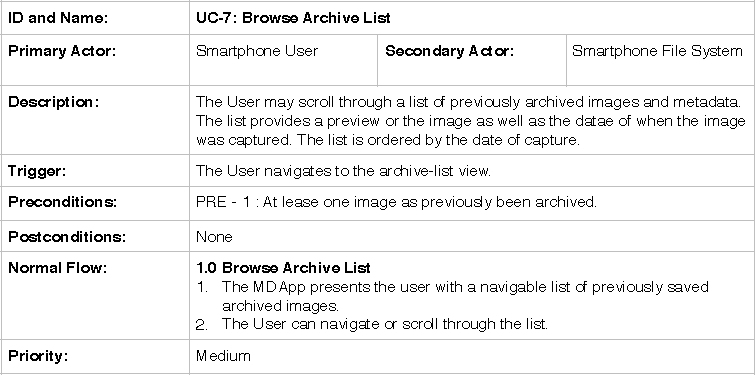
\includegraphics[width=\textwidth]{assets/requirements/uc/usecase_07.pdf}
            \caption{UC-7}
            \label{fig:uc-7}
        \end{table}
        \begin{table}[H]
            \centering
            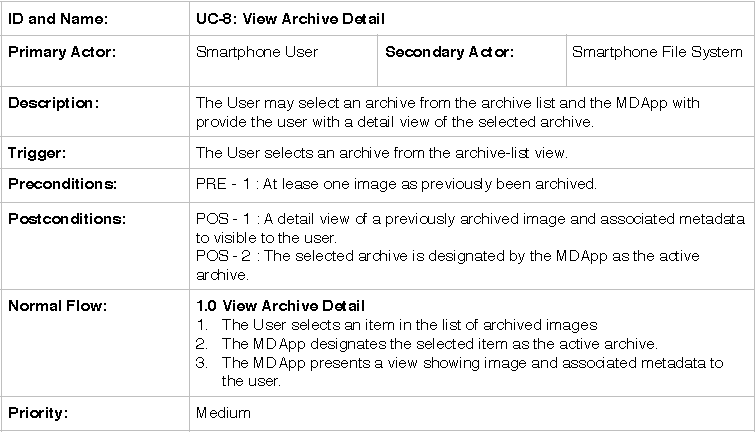
\includegraphics[width=\textwidth]{assets/requirements/uc/usecase_08.pdf}
            \caption{UC-8}
            \label{fig:uc-8}
        \end{table}
        \begin{table}[H]
            \centering
            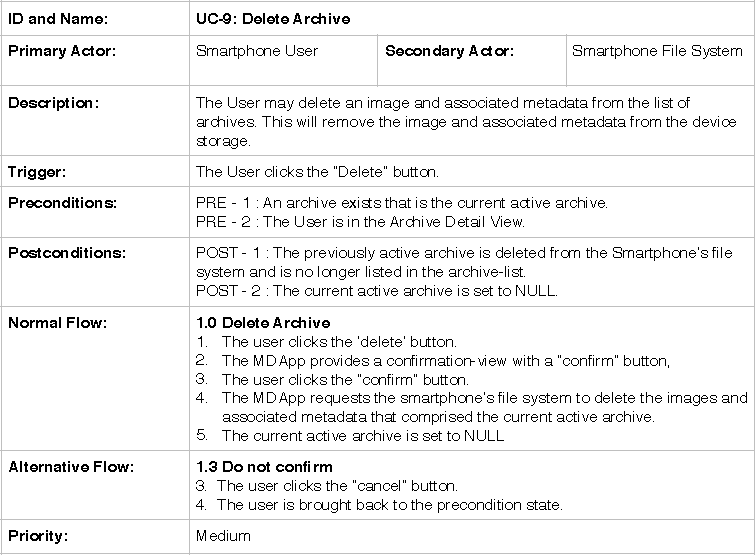
\includegraphics[width=\textwidth]{assets/requirements/uc/usecase_09.pdf}
            \caption{UC-9}
            \label{fig:uc-9}
        \end{table}
        \begin{table}[H]
            \centering
            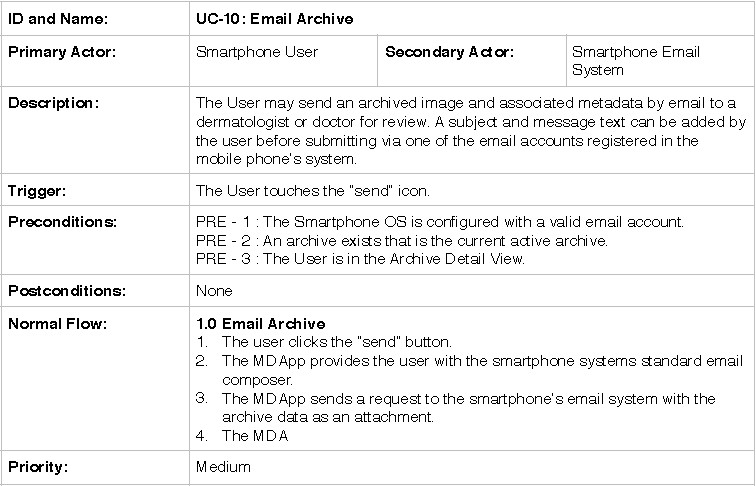
\includegraphics[width=\textwidth]{assets/requirements/uc/usecase_10.pdf}
            \caption{UC-10}
            \label{fig:uc-10}
        \end{table}



\section{Software Requirements Specification}

    \subsection{Introduction}
        \subsubsection{Purpose}

            The Software Requirements Specification will describe the functional and nonfunctional requirements of the Melanoma Detection App. It is meant to be a guideline for developers who will be implementing the mobile application.

    \subsection{Overall Description}
        
        \subsubsection{Product Perspective}

            The Melanoma Detect App will provide the user with a risk assessment of a skin lesion. The App will guide the user through the process of capturing an image and confirming the correct recognition of the boundary of the lesion. Once confirmed the App will analyse the visual features of the lesion based on dermatological rules and provide the user with an initial risk assessment.

    The App should help motivate the user to make an appointment with a dermatologist when a significant risk has been detected. It is not meant to replace the need to visit a dermatologist though.


            \begin{figure}[H]
                \centering
                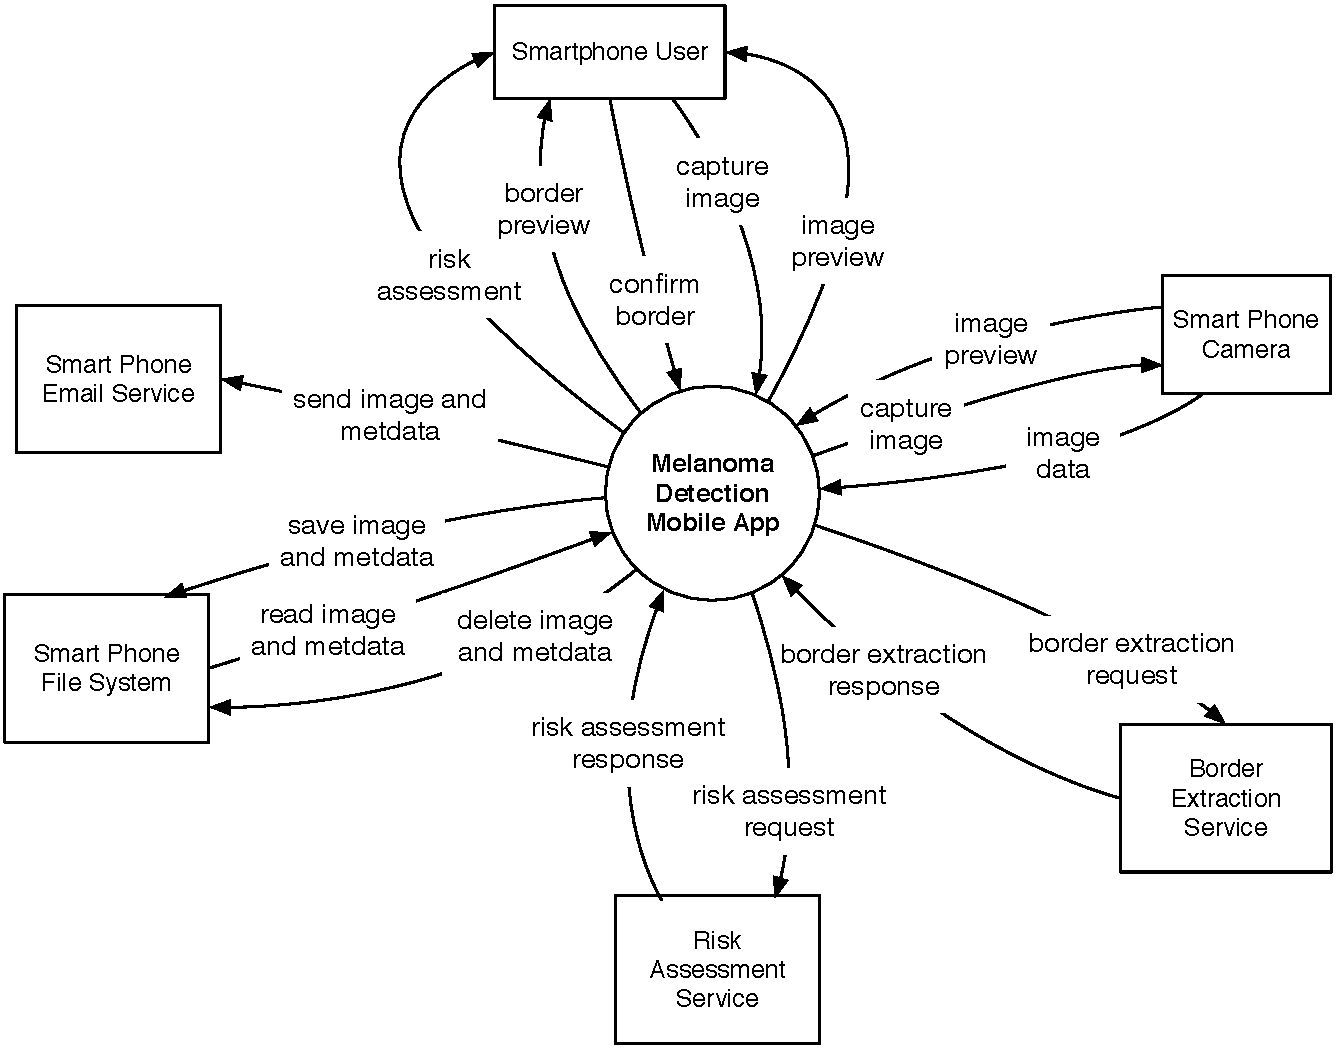
\includegraphics[width=\textwidth]{assets/requirements/ContextDiagram.pdf}
                \caption{Context Diagram of the Melanoma Detection App}
                \label{fig:partial_feature_tree}
            \end{figure}


        \subsubsection{User Classes and Characteristics}

            The Melanoma Detection App only has one class of user, the Smartphone User. The Smartphone User has one or several skin lesions that she or he is worried about.
The Smartphone User is not expected to have any technical or dermatological expertise.

        \subsubsection{Operating Environment}

                    \noindent
                    \begin{itemize}[leftmargin=*]
                        \item[]  \textbf{OE-1} : The Mobile App shall operate on the following platforms: Android OS (minumum v.5.2.2) and iOS (minumum v.9.3)

                    \end{itemize}


        \subsubsection{Design and Implementation Constraints}

                    \noindent
                    \begin{itemize}[leftmargin=*]
                        \item[]  \textbf{CO-1} : The Border Extraction and Risk Assessment Services shall be implemented on a server in oder to leverage the effort already made with python and python based libraries for image processing and scientific calculations. Wifi access is therefore a requirement for the app to run.
                        \item[]  \textbf{CO-2} : The method for archiving images and risk assessment data will use whatever standard is the most accepted for the relevant platform. i.e. iCloud on iOS.


                    \end{itemize}

        \subsubsection{Assumptions and Dependencies}

                    \noindent
                    \begin{itemize}[leftmargin=*]
                        \item[]  \textbf{AS-1} : It is assumed that the user of the software is also the user of the mobile phone. The software might need to request permission from the user to access the camera or network.

                    \end{itemize}

                    \noindent
                    \begin{itemize}[leftmargin=*]
                        \item[]  \textbf{AS-2} : It is assumed that the user of the software is also the only user of the mobile phone. Therefore no additional measures need be taken to secure the app from other potiential users of the phone. The app will be as secure as the phone itself.

                    \end{itemize}

    \subsection{System Features}
        {\renewcommand{\arraystretch}{1.8}%

        \subsubsection{Capture an Image of a Skin Lesion}
            \paragraph{Description}

            The MDApp allows the Smartphone User to capture an image of a skin lesion.

            \paragraph{Functional Requirements}



                \begin{longtable}[H]{ >{\bfseries}l >{\bfseries}l >{\bfseries}l p{8.5cm} l }

                    \hline
                    & \multicolumn{2}{>{\bfseries}l}
                    {Image.Capture:} & \textbf{Capture image using camera}  \\

                    & & .Preview: &  The App must provide the User with a realtime preview of the camera input. It will include some visual indicators that help the user capture an optimal image. \\

                    & & .Trigger: & The User will trigger the capture when he or she decides the realtime preview is optimal. \\

                    & & .Response: & The App must be able to capture a still image from the camera when the User pushed the capture button. The image will be saved in a standard image format on the phone’s file system. \\

                    & & .Display: & The App will present the image to the user on the device’s screen. \\

                    \hline
                \end{longtable}


        \subsubsection{Extract the Border of a Skin Lesion}

            \paragraph{Description}

            In oder to be able to properly analyse the skin lesion image, the MDApp must be able to distinguish pixels that belong to the lesion from pixels that belong to the healthy skin area surrounding the lesion.

            \paragraph{Functional Requirements}

                \begin{longtable}[H]{ >{\bfseries}l >{\bfseries}l >{\bfseries}l >{\bfseries}l p{8.5cm} l }

                    \hline
                    & \multicolumn{3}{>{\bfseries}l}
                    {Border.Extract:} & \textbf{Calculate border of skin lesion}  \\

                    & & \multicolumn{2}{>{\bfseries}l}{.Calculate:} &
                    The App sends a captured image as a request to the Border Extraction Service. When the service has completed the calculation the results of the border calculation are provided by the service to the App.
                    \\

                    & & & .NA & %TODO
                    \\

                    & & & .Err & %TODO
                    \\

                    & & \multicolumn{2}{>{\bfseries}l}{.Display:} &
                    The App will present the results or the border calculation to the User on the device’s screen.
                    \\

                    & & \multicolumn{2}{>{\bfseries}l}{.Promt:} & The App will prompt the User to confirm that the border was precisely calculated. \\

                    & & \multicolumn{2}{>{\bfseries}l}{.Response:} & The User can confirm or cancel the border. \\

                    \hline
                \end{longtable}


        \subsubsection{Calculate the Risk Assessment Skin Lesion}

            \paragraph{Description}

            The MDApp sends the skin lesion image and border data as a request to the Risk Assessment Service.

            \paragraph{Functional Requirements}
                \begin{longtable}[H]{ >{\bfseries}l >{\bfseries}l >{\bfseries}l p{8.5cm} l }

                    \hline
                    & \multicolumn{2}{>{\bfseries}l}
                    {Risk.Assessment:} & \textbf{Calculate risk assessment of lesion image}  \\

                    & & .Calculate: &
                    The App sends a captured image and border data as a request to the Risk Assessment Service. When the service has completed the calculation the results of the risk assessment are provided by the service to the App.
                    \\

                    & & .Display: &
                    The App will present the results or the risk assessment calculation to the User on the device’s screen.
                    \\
                    \hline
                \end{longtable}


        \subsubsection{Create, Modify, and Delete Metadata}

            \paragraph{Description}

            The Smartphone User can add metadata to a captured image. This can include the location on the body that the image was captured from, date of capture, and a text description. This metadata can be associated with an image so that it can be used at a later data for comparison and review.

            \paragraph{Functional Requirements}
                \begin{longtable}[H]{ >{\bfseries}l >{\bfseries}l >{\bfseries}l p{8.5cm} l }

                    \hline

                    & \multicolumn{2}{>{\bfseries}l}
                    {Metadata.Location:} & \textbf{Specify the lesion’s location on body}  \\

                    & & .Display: &
                    The MDApp will present an image of the human body to the Smartphone User.
                    \\

                    & & .Promt: &
                    The MDApp will prompt the Smartphone User to select or zoom in on a location on the image of the human body.
                    \\

                    & & .Response: &
                    The selected location will be stored as metadata associated with the image of the lesion.
                    \\
                    \hline

                    & \multicolumn{2}{>{\bfseries}l}
                    {Metadata.Text:} & \textbf{Add metadata describing lesion}  \\

                    & & .Display: &
                    The MDApp will present a text field in which the Smartphone User may enter, edit, or delete text.
                    \\


                    & & .Response: &
                    The entered text will be stored as metadata associated with the image of the lesion.
                    \\

                    \hline
                \end{longtable}


        \subsubsection{Save, View, Edit, Delete and Email Archive}


            \paragraph{Description}

            The Smartphone User can browse a list of previously analysed and saved images (archives). From the list, an image may be selected by the Smartphone User to view in more detail. When selected the MDApp will present the saved image, border, risk assessment, and associated metadata to the Smartphone User for review. An archive from the list may also be deleted or sent as an email.

            \paragraph{Functional Requirements}
                \begin{longtable}[H]{ >{\bfseries}l >{\bfseries}l >{\bfseries}l p{8.5cm} l }

                    \hline

                    & \multicolumn{2}{>{\bfseries}l}
                    {Archive.Save:} & \textbf{Save image and metadata as archive}  \\

                    & & .Display: &
                    ---
                    \\
                    \hline
                    & \multicolumn{2}{>{\bfseries}l}
                    {Archive.Browse:} & \textbf{Browse list of archived images}  \\

                    & & .Display: &
                    The MDApp will present the Smartphone User with a list of saved archive images.
                    \\
                    \hline
                    & \multicolumn{2}{>{\bfseries}l}
                    {Archive.Select:} & \textbf{Select archived image to view or edit}  \\

                    & & .Display: &
                    The MDApp will present the Smartphone User with a detail view of the selected archived image and associated metadata.
                    \\
                    & & .Edit: &
                    The MDApp will present a text field in which the Smartphone User may enter, edit, or delete text.
                    \\
                    & & .Delete: &
                    The MDApp will present a text field in which the Smartphone User may enter, edit, or delete text.
                    \\
                    & & .Email: &
                    The MDApp will present a text field in which the Smartphone User may enter, edit, or delete text.
                    \\


                    \hline
                \end{longtable}
}



    \subsection{Data Requirements}
        
        \subsubsection{Logical Data Model}

            \begin{figure}[H]
                \centering
                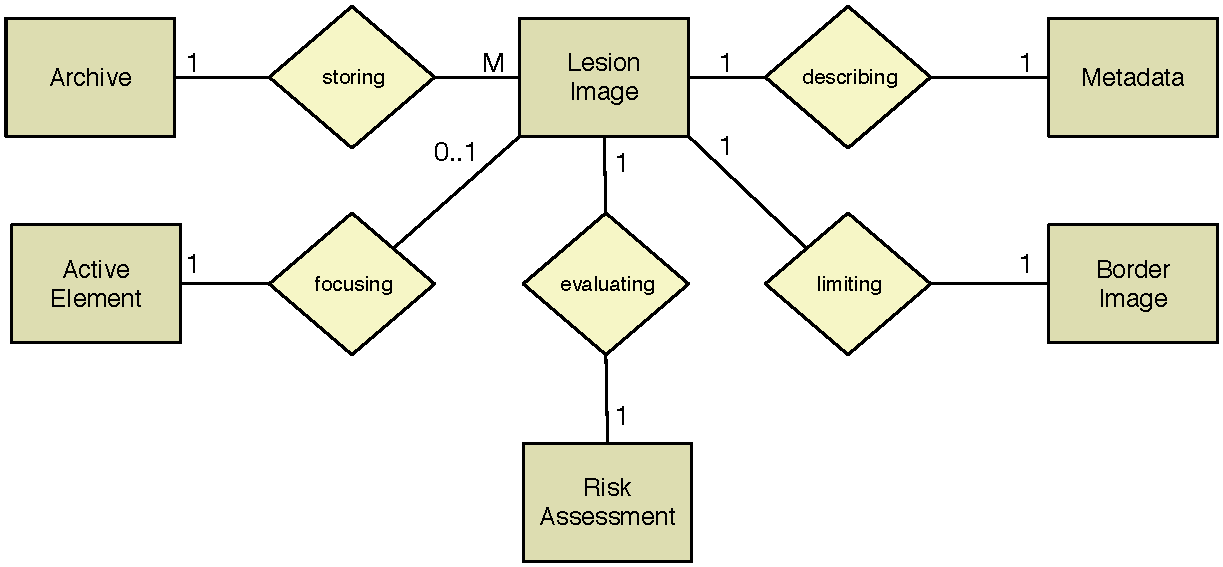
\includegraphics[width=\textwidth]{assets/requirements/EntRel.pdf}
                \caption{Patial data model of the Melanoma Detection App}
                \label{fig:partial_data_model}
            \end{figure}


        \subsubsection{Data Dictionary}

                \begin{longtable}[H]{ | l | p{3.0cm} | p{2.5cm} | p{1.0cm} | p{2.5cm} | }

                    \hline
                    \textbf{Data element} & \textbf{Description} & \textbf{Componsition or data type} & \textbf{Length} & \textbf{Values} \\ \hline

                    \hypertarget{lesion_image}{Lesion Image} & reference to the captured image &

                        \specialcell[t]{Image ID
                           \\ + File Path
                           \\ + Creation Date
                        }

                     & & \\ \hline

                    Image ID & unique identifier for an image &
                    integer & 11 & system-generated sequential integer beginning with 1 \\ \hline

                    File Path & location of a file on the file system &
                    string & 256 &  \\ \hline

                    Creation Date & date and time that a file was created &
                    DDMMYYYYHHSS &  &  \\ \hline

                    Metadata & information describing the lesion and it's location &

                        \specialcell[t]{\hyperlink{lesion_image}{Lesion Image}
                           \\ + Lesion Description
                           \\ + Lesion Location
                        }

                     & & \\ \hline

                    Lesion Description & User defined text that describes the lesion &
                    alphanumeric &  &  \\ \hline

                    Lesion Location & information describing the lesion location on the body &

                        \specialcell[t]{\hyperlink{lesion_image}{Lesion Image}
                           \\ + Body Location ID
                           \\ + X Coordinate
                           \\ + Y Coordinate
                        }

                     & & \\ \hline


                    Body Location ID & id of a region on the body &
                    integer & 2 & TBD \\ \hline

                    X Coordinate & x coordinate of the lesion in the region specified by the body location id &
                    integer & 128 &  \\ \hline

                    Y Coordinate & y coordinate of the lesion in the region specified by the body location id &
                    integer & 128 &  \\ \hline

                    Border Image & data that defines the outline of the lesion area &

                        \specialcell[t]{\hyperlink{lesion_image}{Lesion Image}
                           \\ + File Path
                           \\ + Creation Date
                        }

                     & & \\ \hline

                    Risk Assessment &  &

                        \specialcell[t]{\hyperlink{lesion_image}{Lesion Image}
                            \\ + Assessment Date
                            \\ + Version Number
                            \\ + SFA Major
                            \\ + SFA Minor
                            \\ + Border Irregularity
                            \\ + Color Score
                            \\ + \hyperlink{tds_score}{TDS Score}
                        }

                    & & \\ \hline

                    Assessment Date & date and time that the risk assessment was calculated &
                    DDMMYYYYHHSS &  &  \\ \hline

                    Version Number & version number of the risk assessment service software &
                    integer & 4 &  \\ \hline

                    SFA Major & measure of symmetry of the lesions major axis &
                    integer & 3 & 0 - 360 \\ \hline

                    SFA Minor & measure of symmetry of the lesions minor axis &
                    integer & 3 & 0 - 360 \\ \hline

                    Border Irregularity & measure of irregulatiry of the lesion's border &
                    integer & 1 & 0 - 8 \\ \hline

                    Color Score & number of specific colors found in the lesion's image &
                    integer & 1 & 0 - 8 \\ \hline

                    \hypertarget{tds_score}{TDS Score} & weighted linear combination of the image features summarizing the risk assessment  &
                    float &  & 1 - 8.9 \\ \hline

                    Archive &  &

                        \specialcell[t]{Archive ID
                            \\ + \hyperlink{lesion_image}{Lesion Image}
                            \\ + Metadata
                            \\ + Border
                            \\ + Risk Assessment
                            \\ + Archive Date
                        }

                     & & \\ \hline


                    Color Score & number of specific colors found in the lesion's image &
                    integer & 1 & 0 - 8 \\ \hline

                \end{longtable}


        \subsubsection{Data analysis}
            \paragraph{CRUD Matrix}

                \begin{figure}[H]
                    \centering
                    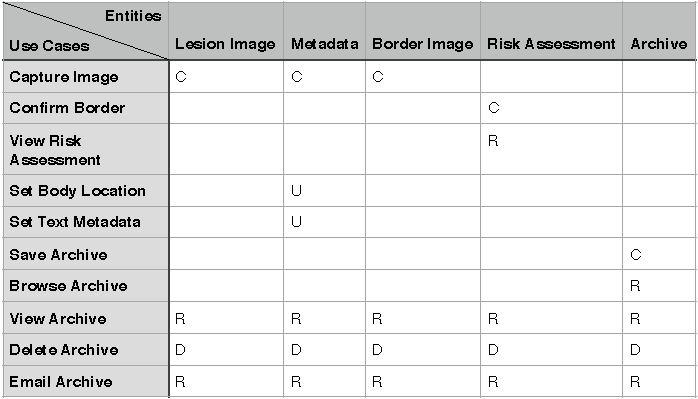
\includegraphics[width=\textwidth]{assets/requirements/CRUD.pdf}
                    \caption{CRUD matrix for Melanoma Detection App}
                    \label{fig:crud}
                \end{figure}

        \subsubsection{Reports}
            \paragraph{Email Report}
                When the Smartphone User chooses to send an archive as an email, the data must be flattened into a format that is email compatible. The body of the email will be an html formated document that displays the lesion image, the calculated border, the risk assessment data and the associated metadata.




    \subsection{External Interface Requirements}
        \subsubsection{User Interfaces}

        \begin{itemize}[leftmargin=1.4cm]
            \item[UI-1 :] The UI shall guide the Smartphone User sequentially through the process of capturing and analysing an image. The Smartphone User should not be able to jump through states in wrong sequence.
            \item[UI-2 :] The UI shall allow the Smartphone User to capture an image easily, using only one hand.
            \item[UI-3 :] When waiting for a process to finish or a response from an online server the UI should visually indicate that it is waiting for a long process. ( i.e. throbber, spinning wheel, progress indicator )
            \item[UI-4 :] The UI shall allow the Smartphone User to select her or his preferred language ( i.e. localisation )
            \item[UI-5 :] The UI shall conform to native UI standards as much as possible.
            \item[UI-6 :] Unless in conflict with UI-5 the UI shall have the same components across multiple platforms.

        \end{itemize}

\subsubsection{Software Interfaces}

    \paragraph{Smartphone Camera }

        The MDApp will interface with the Smartphone's camera hardware via the systems camera API.

        \begin{itemize}[leftmargin=1.4cm]
            \item[SI-1.1 :] The MDApp shall activate the camera when needed and be able to receive a live preview stream from the camera.
            \item[SI-1.2 :] If the native API allows, the MDApp should set to camera’s focus mode to Macro.
            \item[SI-1.3 :] If the native API allows, the MDApp should register a call back to be informed when the camera’s autoFocus has focused.
            \item[SI-1.4 :] The MDApp shall signal the camera to capture the highest resolution image possible when the Smartphone User triggers an image capture event.

        \end{itemize}

    \paragraph{Smartphone File System}

        Captured images and Border Analysis images must be stored on the Smartphone File System in such a manner so that they are accessible by the Smartphone User in the native methods. The native file access, file handling, and backup methods for the respective Smartphone platform shall apply to files created and captured by the MDApp

        \begin{itemize}[leftmargin=1.4cm]
            \item[SI-2 :] The MDApp will save files to the Smartphone's native file system.

        \end{itemize}

    \paragraph{Smartphone Email Service}

            \begin{itemize}[leftmargin=1.4cm]
            \item[SI-3 :]

        \end{itemize}

\subsubsection{Communication Interfaces}

    \paragraph{Border Extraction Service }

        The Border Extraction Service is an online web based service that the MDApp can communicate with for the purpose of extracting the precise border information from a captured image of a skin lesion.

        \begin{itemize}[leftmargin=1.4cm]
            \item[CI-1.1 :] The MDApp will upload a captured skin lesion image to a web-based Border Extraction Service. The method for uploaded as part of a multipart/form-data html POST method.
            \item[CI-1.2 :] The MDApp will receive a confirmation from the service as JSON, including an id that will be used to poll the service for progress.
            \item[CI-1.3 :] The MDApp will poll the online service regularly, the service will indicated that the Border Extraction processes is in progress or has finished, in which case it will also include the url where the border image can be downloaded.
            \item[CI-1.4 : ] The MDApp will download the border data image from the Border Extraction Service

        \end{itemize}

    \paragraph{Risk Assessment Service }

        The Risk Assessment Service is an online web based service that the MDApp can communicate with for the purpose of evaluating the risk of a skin lesion being a melanoma.

        \begin{itemize}[leftmargin=1.4cm]
            \item[CI-2 :] The MDApp will upload a captured skin lesion image to a web-based Border Extraction Service. The method for uploaded as part of a multipart/form-data html POST method.

        \end{itemize}

    \subsection{Quality Attributes} % TODO
        \subsubsection{External Quality Attributes}

            \paragraph{Installability}

                INST-1 : Installing the MDApp shall not require any special instructions other than those a normal Smartphone User would expect.


            \paragraph{Integrity}

                INTE-1 : Any data created by the Smartphone User through use of the MDApp shall be backup-able through whatever native backup solutions the native platoform offers.

                INTE-2 : Data and state shall be persisted, so that when reopened, the MDApp will have the same state as when it was last closed.
                INTE-3 : Data and state shall be persisted, so that no data is lost when the MDApp is updated.

            \paragraph{Useability}

        \subsubsection{Internal Quality Attributes}

            \paragraph{Modifiability}

                MODI-1

            \paragraph{Portability}

                PORT-1 : The MDApp shall have an identical feature set accross all the device platforms it runs on.

            \paragraph{Testability}

                TEST-1 :







